\documentclass[pdf, aspectratio=169, 12pt]{beamer}
\usepackage[]{hyperref, graphicx, siunitx, lmodern, tikz, booktabs, physics, multicol}
\usepackage[mode=buildnew]{standalone}
\usepackage{pdfpc-commands}
\usepackage{pgfplots}
\pgfplotsset{compat=1.16}

\usetheme{Python}

\graphicspath{ {Images/} }

\sisetup{per-mode=symbol}
\usetikzlibrary{calc, patterns, decorations.markings, decorations.pathmorphing, shapes, fit}

%Preamble
\title{Animation and Control}
\author{Jed Rembold}
\date{Nov 13, 2019}

\begin{document}

\begin{frame}{Announcements}
	\begin{itemize}
		\item Homework
			\begin{itemize}
				\item Homework 10 posted! (Actually this time!)
				\item I'm still working on getting HW9 graded
			\end{itemize}
		\item Project info coming Friday
			\begin{itemize}
				\item Poll will be going out to you to get some feedback on potential groups
			\end{itemize}
		\item Polling: \nolinkurl{rembold-class.ddns.net}
	\end{itemize}
\end{frame}

\begin{frame}[fragile]{Review Question}
	\begin{columns}
		\column{0.5\textwidth}

		\vspace{3mm}
		Which block of code to the right will produce the arrangement of axes below?
		\begin{center}
			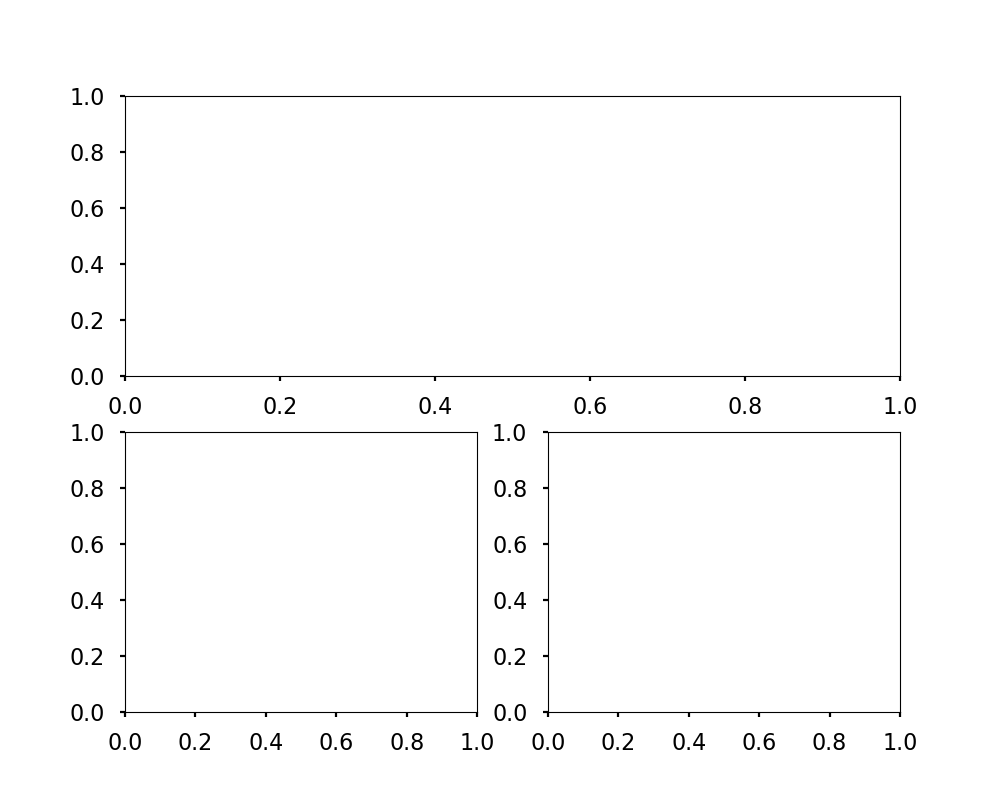
\includegraphics[width=\textwidth]{RQ13.png}
		\end{center}
		\column{0.5\textwidth}
		\vspace{-5mm}
		\begin{poll}
		\item
			\begin{pythoncode}
				ax1 = f.add_subplot(222)
				ax2 = f.add_subplot(221)
				ax3 = f.add_subplot(212)
			\end{pythoncode}

		\item
			\begin{pythoncode}
				ax1 = f.add_subplot(223)
				ax2 = f.add_subplot(221)
				ax3 = f.add_subplot(122)
			\end{pythoncode}

		\item
			\begin{pythoncode}
				ax1 = f.add_subplot(224)
				ax2 = f.add_subplot(223)
				ax3 = f.add_subplot(211)
			\end{pythoncode}

		\item
			\begin{pythoncode}
				ax1 = f.add_subplot(213)
				ax2 = f.add_subplot(211)
				ax3 = f.add_subplot(222)
			\end{pythoncode}
		\end{poll}
	\end{columns}
\end{frame}

\begin{frame}{Grouping Image Components}
	\begin{itemize}
		\item Drawings make an easy way to use classes to make more complicated objects!
		\item Break the process of creating the drawing into multiple methods
			\begin{itemize}
				\item Maybe one to create the parts of the image
				\item One to color the parts of the image
				\item One to draw the parts of the image
			\end{itemize}
		\item Will be very useful for later creating movement and animation
			\begin{itemize}
				\item Can add motion, physics, etc to each object
			\end{itemize}
	\end{itemize}
\end{frame}

\begin{frame}{Adding Motion}
	\begin{itemize}
		\item Can use \pyi{.move(dx,dy)} to move a graphical element by a $dx$ and $dy$
		\item $dx$ and $dy$ are a displacement!
			\begin{itemize}
				\item Shift from the current location
				\item You can not directly tell it to move to a particular point
					\begin{itemize}
						\item Would need to find the difference between where it is at and where you want it to go.
					\end{itemize}
			\end{itemize}
	\end{itemize}
\end{frame}

\begin{frame}{Animation: Method 1}
	\begin{itemize}
		\item Continuous motion achieved through repeated \pyi{.move} calls
		\item One method would be inside a loop
		\item You \alert{need} some way to regulate the speed of the movement
			\begin{itemize}
				\item The drawing will not be able to visibly keep up with Python otherwise
				\item Can use \pyi{update()} in loops
					\begin{itemize}
						\item Will force an update to the motion at that point
						\item Can pass in a rate for the number of times it will update per second
					\end{itemize}
			\end{itemize}
	\end{itemize}
\end{frame}

\begin{frame}{Animation: Method 2}
	\begin{itemize}
		\item Often nice to bundle movement commands into a class, where it is cumbersome to call that method each time in the loop
		\item Might also want movement to still be happening while the program waits for some mouse or key press
		\item Can use a recursive call which tells the graphics window to call this same move method again after a specified delay.
			\begin{itemize}
				\item Use \pyi{<window obj>.after(<delay>, <function>)}
				\item The window will figure out the timing to move the requested objects when it has a spare moment
			\end{itemize}
	\end{itemize}
\end{frame}

%\begin{frame}{Better Key and Mouse Control}
	%\begin{itemize}
		%\item Two ways of getting input
			%\begin{itemize}
				%\item Blocking Methods:
					%\begin{itemize}
						%\item Mouse: \pyi{.getMouse()}
						%\item Key: \pyi{.getKey()}
					%\end{itemize}
				%\item Non-Blocking Methods:
					%\begin{itemize}
						%\item Mouse: \pyi{.checkMouse()}
						%\item Key: \pyi{.checkKey()}
					%\end{itemize}
			%\end{itemize}
		%\item Mouse will return the coordinates clicked as a \pyi{Point} object
		%\item Key will return the key pressed as a string
		%\item Consider printing those values to the screen if you are confused about what they are doing!
	%\end{itemize}
%\end{frame}





\end{document}

